\documentclass{article}

% list of necessary packages
\usepackage[utf8]{inputenc}
\usepackage{amsfonts, amsmath, amssymb, amsthm}
\usepackage{nicefrac}
%\usepackage{fullpage}
\usepackage[section]{placeins}
\usepackage{url}
\usepackage[english]{babel}
\usepackage{titling}

% list of optional packages
\usepackage{graphicx, subfig}
\usepackage{algpseudocode}
\usepackage{changepage}
\usepackage{xcolor,soul}

% paragraph spacing
\setlength{\parindent}{0pt}
\setlength{\parskip}{8pt}


% table spacing
\def\arraystretch{1.2}


% configuration of header and footer
\pagenumbering{arabic}
\usepackage{fancyhdr}
\pagestyle{fancy}
\fancyhf{}
\fancyhead[C]{
	{\large {\theauthor} }
}
\fancyfoot[C] {
    { {\thepage} }
}
\renewcommand{\headrulewidth}{0pt} % 0.4pt lined
\setlength{\headheight}{14pt}
\setlength{\headsep}{16pt}

\usepackage{listings}


\begin{document}
    % config
    \title{Lab: Efficient Algorithms}
    \author{Rademacher, Loka}
    \date{\today}

    % super nice header
    \thispagestyle{empty}
    \begin{center}
        \noindent
        \makebox[0pt][l]{Final Report}%
        \makebox[\textwidth][c]{\textbf{University of Bonn}}%
        \makebox[0pt][r]{\thedate}


        \noindent
        \centerline{\huge \sc \thetitle}

        \vspace*{-2pt}

        \noindent
        \centerline{\large {\theauthor}}
    \end{center}



    \section{Introduction}

    The goal of the lab \textit{Efficient Algorithms and Selected Problems} was to engage with a given problem and state-of-the-art algorithms which solve them really well. The problem we are given was path finding on grid graphs and the main algorithm was jump point search with the pruning technique bounding boxes.

    We wrote an implementation of this algorithm and some similar ones which are frequently used to compare them amongst themselves. The similar algorithms are different variants of jump point search and the well known A star algorithm. On top of implementing the algorithm we have added some tools to visualize the algorithms and to benchmark our algorithm variants. Our actual implementation is independent from the visualization so that the algorithm is also applicable outside of the visualization environment. The purpose of the visualization environment is to help to understand the algorithm.

    The source code of the implementation will be available at \url{https://github.com/dhaunac/lab-jump-point-search} after the final presentation as all our other work relating to the lab.



    \section{Path finding on grid graphs}

    Our problem setting is to find the shortest path on a grid graph $G$. The drawing of a grid graph forms a regular tiling in the Euclidean space. Each tile which touches another one in the drawing is connected in the graph trough an edge. We refer to the missing tiles in the drawing as obstacles. The cost of each edge is determined only by the direction. An orthogonal edge has cost of $1$ and a diagonal edge has cost of $\sqrt{2}$.

    For that cost function on Euclidean grids there are a number of so called heuristic functions. The heuristic function estimates the cost of the total way between two vertices. The existence of such a function helps our algorithms to decide whether a walked path has led to a good or bad vertex. Formal speaking a heuristic function is a function $h : V \times V \rightarrow \mathbb{R}$. The constraint any heuristic function has to fulfill is the admissibility. A admissible heuristic is never overestimating the cost between two points, i.e. for all $a, b \in G$ it holds $h(a, b) \leq c(a,b)$. The other constraint is consistency which says that the heuristic cost between two points is not higher that the heuristic from $a$ to a neighbor of $b$ and the cost from that neighbor to $b$, i.e. $\forall a, b, c: h(a, b) \leq h(a, c) + c(c, b)$. A consistent heuristic is also admissible. If we would use a heuristic which is not admissible then all of our algorithms would not return a correct shortest path. A consistent heuristic improves our running time. All the heuristics we regarded are admissible.

    Every problem instance has given two additional points. One of it is the start point and the other the goal point of that instance. This now yields a 4-tuple of grid graph $G$, start point $s$, goal point $g$ and heuristic function $h$. Now the algorithm has to determine the shortest path from start to goal point~\cite{DBLP:conf/aaai/HaraborG11}.



    \section{Algorithms}
    \label{sec:algorithms}

    The implementation of the following algorithms was the main aspect of the lab task. At first we give an outline of the algorithms so that the reader is familiar with those before discussing implementation issues.

    \subsection{A star search $A^\star$ }

    In this section we will discuss the $A^\star$ search algorithm~\cite{Astar}. The algorithm is basically a natural extension of the Dijkstra algorithm. It consist of an open list of next candidate vertices and a closed list of already processed vertices. The open list is usually some kind of priority queue and the closed list is a set.

    The algorithm then gets a graph, a cost function and an admissible heuristic function as input. It starts with adding the start node into the open list and then processes a main loop. The main loop extracts the vertex $v$ of the open list with minimum cost and expands all its adjacent vertices. The expansion step checks whether the vertices are not in the closed list and if so adds it to the open list with a cost value of the sum from the cost to $v$ and the cost from $v$ to the expanded point. After that add $v$ to the closed list and repeat the main loop. The minimum cost is the sum of the cost value and the heuristic from that point to the goal node. So while progressing closer to the goal point the minimum cost might decrease.

    \subsection{Jump point search $JPS$}

    Now we will discuss the first paper~\cite{DBLP:conf/aaai/HaraborG11}. At first take a look at figure~\ref{fig:symmetricpath} where we can see the behavior of the $A^\star$ algorithm. So for given points there is a high likelihood that there exist a lot of symmetric paths. By symmetric paths we refer to paths which are equal in terms of the number of orthogonal and diagonal edges.

    \begin{figure}[!htb]
        \centering
        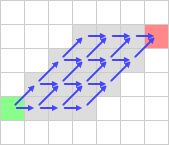
\includegraphics{figures/symmetricpath.png}
        \caption{Different possibilities for the shortest path in $A^\star$ \cite{JPSexplained}}
        \label{fig:symmetricpath}
    \end{figure}

    At this point the improvements of jump point search start. The algorithm is built in a way to avoid all of those symmetric paths. This is done by defining a priority to each edge so there is one path who is preferred before any else. Once a path has been found any other will not be explored anymore. $JPS$ will always prefer the diagonal steps and thus takes those before any orthogonal edge. Additionally the algorithm ignores some edges which would lead to a non-optimal path by examining the previous edge direction. This results in a local pruning technique. To be more precise we will have a closer look on that. When we look at the previous direction we already know its a bad move to take the inverse direction, because this is redundant walking. Similar arguments can be applied to every direction not going forward or forward sideways, since those are the only directions resulting in vertices which could not be reached any better.

    \begin{figure}[!htb]
        \centering
        \subfloat[orthogonal moves \cite{JPSexplained}.]{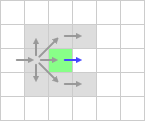
\includegraphics[width=0.4\textwidth]{figures/sm.png}\label{fig:sm}}
        \hfill
        \subfloat[diagonal moves.]{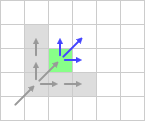
\includegraphics[width=0.4\textwidth]{figures/dm.png}\label{fig:dm}}
        \caption{JPS behavior with no obstacles in sight \cite{JPSexplained}.}
    \end{figure}

    So for every point we might have the case that the pruning will leave is with just one expansion node. So instead of pushing those kind of vertices to the open list we just push those points which have more than one expansion possibilities, because that is an interesting case which have to be process in a non-trivial way. That behavior can lead to expansion steps between not adjacent vertices also. The skipping of vertices is called a jump. Jump points are all those points where a jump ends and a new jump can be started.

    The most important thing to care about is the modifications for obstacles. The improvements mentioned so far will work properly if there are no obstacles on the path. So for any obstacle encountered the algorithms we have to add other expansion points which offer an alternative since the usual best path is blocked.

    \begin{figure}[!htb]
        \centering
        \subfloat[orthogonal moves \cite{JPSexplained}.]{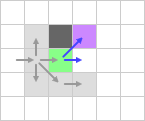
\includegraphics[width=0.4\textwidth]{figures/sm_forced.png}\label{fig:sm_forced}}
        \hfill
        \subfloat[diagonal moves.]{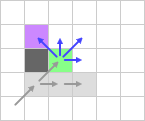
\includegraphics[width=0.4\textwidth]{figures/dm_forced.png}\label{fig:dm_forced}}
        \caption{JPS behavior at encountering obstacles \cite{JPSexplained}.}
    \end{figure}

    \begin{figure}[!htb]
        \centering
        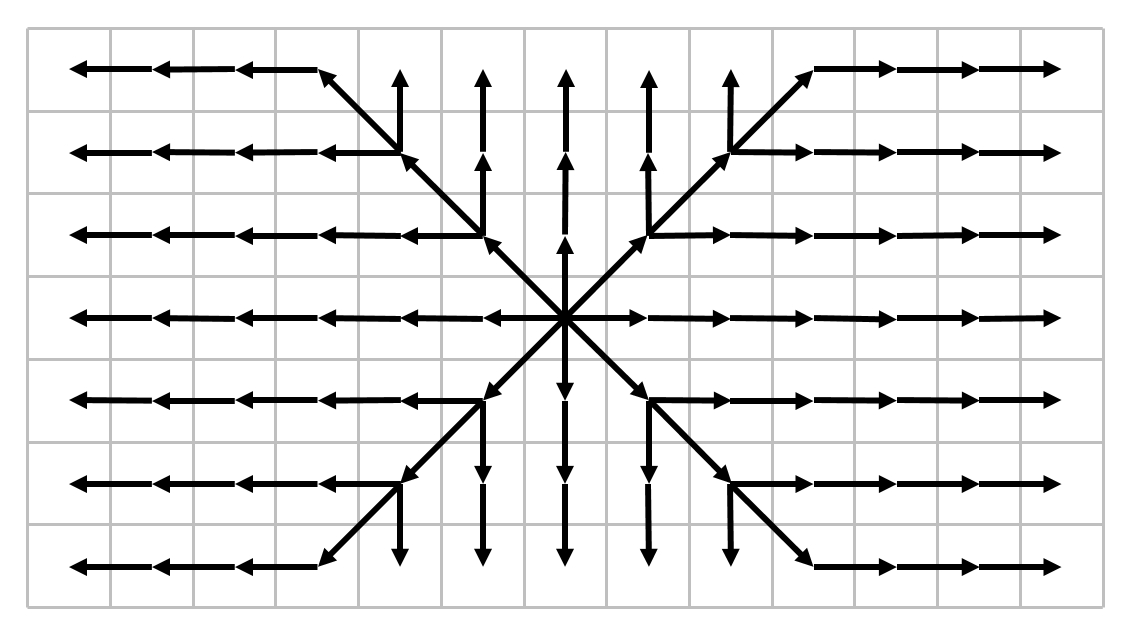
\includegraphics[width=\textwidth]{figures/jps_strategy.png}
        \caption{Natural order of exploration in $JPS$}
        \label{fig:pathorder}
    \end{figure}



    \subsection{Jump point search Improvements $JPS^+$}

    There is an improvement of $JPS$ called $JPS^+$~\cite{DBLP:conf/aips/HaraborG14}. Its a preprocessing technique to reduce the work of $JPS$ during run.

    Preprocssing
    Explore Schritt von JPS in einer lookup table



    \subsection{Bounding boxes pruning $BB$}

    Bounding boxes is a pruning technique that can be applied to lot of different path finding algorithms~\cite{DBLP:conf/aaai/RabinS16}. The pruning requires some preprocessing which can be done offline, i.e. before the actual start and goal point are known.

    For each pair of points and direction we have a dedicated bounding box. This box consists of all points which are can be reached optimally on a path from that given point. The box itself is the smallest geometric container, in this case a rectangle, to have every of those points inside. This implies that any point outside the box will be pruned since they will not help finding an optimal path.

    The bounding depends on the underlying algorithms, in case of $A^\star$ and $JPS$ it is sufficient to have minimum and maximum values for the X and Y coordinates. For $A^\star$ we can determine a predecessor $p$ for the point $v$ by inverting the direction. Then the bounding box of the point consists of all points which have a shortest path from $p$ to those points using $v$ as intermediate point. For $JPS$ we can go even further and use the knowledge of our jump points and natural ordering. Here the pruning will be even more effective which can be observed in our visualization of the algorithm.

    \begin{figure}[!htb]
        \centering
        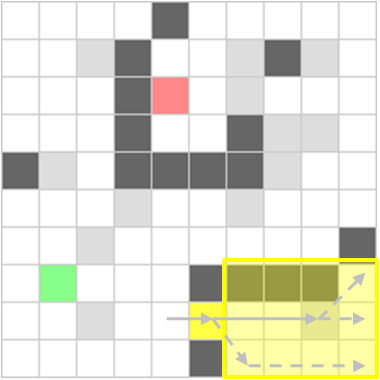
\includegraphics{figures/bounding_boxes.png}
        \caption{Visualization of bouding boxes.}
        \label{fig:bounding_boxes}
    \end{figure}




    \section{Implementation}

    \subsection{Application Core}

    The main goal and therefore the most important part of the lab work was to implement our algorithms. Our core offers an interface for external usage. One can use it as a library for any kind of application. We split up every choice of algorithm settings in a way everything can be combined as needed. The algorithm settings have the main point algorithmic structure, heuristic function and grid graph movement rules. The structure is the basis of everything, here you can choose between every algorithm described above. The algorithms are $A^\star$, $JPS$ and $JPS^+$. Everyone can be additionally combined with bounding boxes pruning to speed up search. The heuristic functions can be chosen from one of the commonly used ones which are Manhattan distance, Euclidean distance or Grid distance. Grid distance is the shortest possible distance on any grid graph where no obstacle hinders the movement. Its also possible to choose no heuristic function which will for example make $A^\star$ behave like the Dijkstra algorithm. At last one has to choose the movement rule. The decides in which way an algorithm is allowed to move on the grid graph. One option is orthogonal movement where every diagonal edge is forbidden. The other options decide whether edge cutting is allowed. Edge cutting offers an option to use diagonal edges even though part of an obstacle is lying on the way.


    \subsection{Visualization and user interface}

    The visualization is the second substantial aspect of our work. To begin we will explain the basic working of the user interface. At first one can use the \textit{File} menu to load any map. There are a number of different possibilities to create a random map satisfying a specific layout, for example perfect mazes or random rooms connected in a selected way. The next menu is \textit{Edit} where the user can edit the map or change the algorithm settings. We offer $A^\star$, $JPS$, $JPS^+$ and each of them with additional $BB$ pruning. Those algorithms are explained in section~\ref{sec:algorithms}. On top of that one can modify each of those algorithms by choosing a heuristic and a moving rule. The heuristic modification leads into situations where different candidates of the open list will be explored. The change in the moving rule offers interesting observations when used with some kinds of jump point search and shows also the limits of jump point search. Then the user is supposed to pick locations for the start and goal point. Then the algorithm can be run after some prepossessing if necessary. We have separate steps for those actions, so one can easily modify the algorithm settings and see the changes after running the other algorithm settings.

    The visualization will show the result of the algorithms. The red line between the chosen start and goal point indicates the shortest path. We have different colors for points which are in the open list or closed list. Every type of points can be shown or hidden by using the \textit{View} menu.

    The Java implementation is written using JavaFX, the successor of Swing.

    \begin{figure}[!htb]
        \centering
        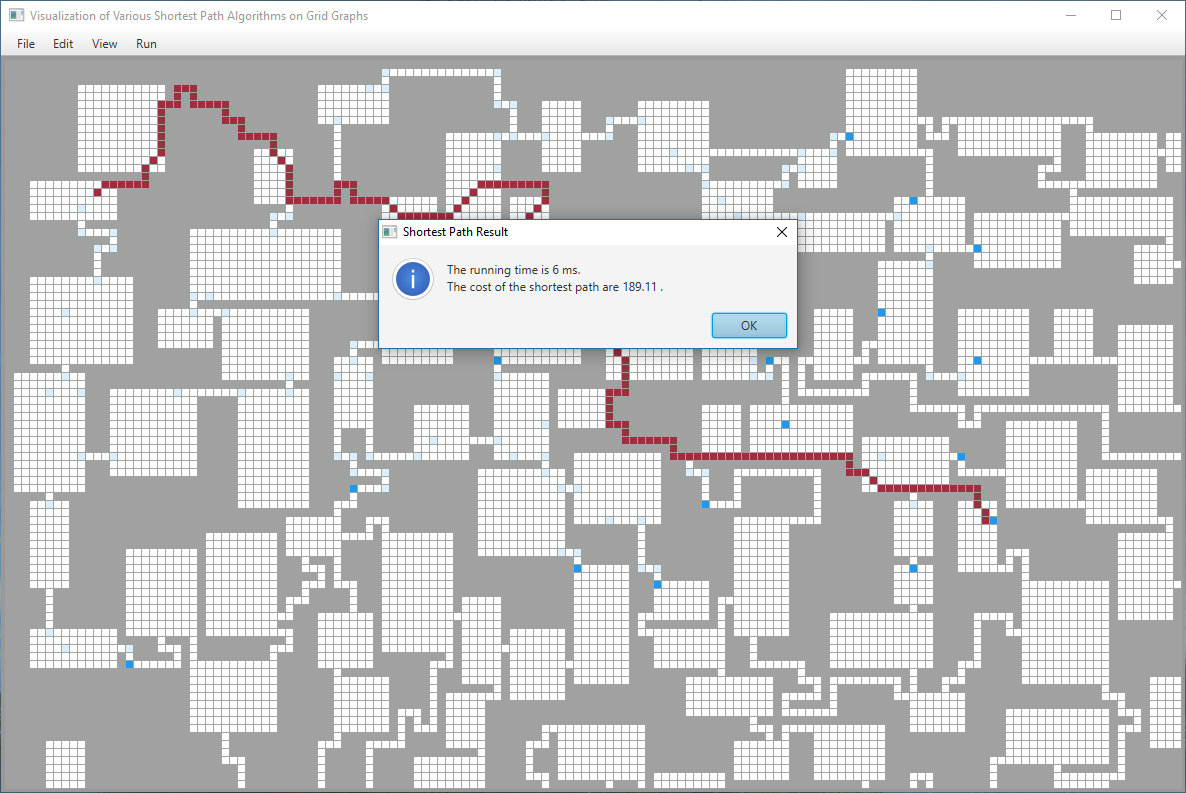
\includegraphics[width=\textwidth]{figures/javafx.png}
        \caption{Screenshot of the user interface.}
        \label{fig:javafx}
    \end{figure}



    \subsection{Benchmarking measurements}

    In addition to the visualization we wrote a benchmark application for terminal usage. This benchmark application could be used by other people who want to find out which algorithm settings is best for their real world application. We used it for a given set of benchmark maps and so called scenarios to find out how other our implementations are. The results of this benchmarking can be found in section~\ref{sec:results}. The usage of the terminal is simple. You can start it by using following command

    \begin{lstlisting}[basicstyle=\small\ttfamily]
      # java -classpath $PATH_TO_JAR$/LabApplication.jar
        terminalapplication.Main $DIR$ $ALGO$
    \end{lstlisting}

    In that command we have three parameters where the name should be self-explaining. The accepted names of algorithms are $astar$, $astarbb$, $jps$, $jpsbb$, $jpsplus$, $jpsplusbb$. The directory has some requirements to be fulfilled. The first is that a directory with that name is a sub directory in both \textit{maps} and \textit{scenarios} directory. In the sub directory in maps there has to be maps with .map suffix and format encoding as in MovingAI \cite{sturtevant2012benchmarks}. The same holds for the sub directory in scenarios, where each file has to have the .scen suffix and appropriate encoding.

    Each map will we processed along with the corresponding scenario file. To benchmark a single map it has to be in its own folder if that is necessary.



    \section{Results}
    \label{sec:results}

    TODO: Hier könnten ein paar Plots stehen aus den benchmark Ergebnissen, die wir haben (?)

    \cite{sturtevant2012benchmarks}


    \bibliographystyle{alpha}
    \bibliography{references}
\end{document}
